\documentclass[11pt, a4paper]{article}

\usepackage[utf8]{inputenc}
\usepackage{geometry}
\usepackage{graphicx}
\usepackage{amsmath}
\usepackage{amssymb}
\usepackage{hyperref}
\usepackage{listings}
\usepackage{xcolor}
\usepackage{booktabs}
\usepackage{float}
\usepackage{caption}
\usepackage{subcaption}
\usepackage{tikz}
\usetikzlibrary{shapes.geometric, arrows, positioning}

\geometry{a4paper, margin=1in}

\hypersetup{
    colorlinks=true,
    linkcolor=black,
    filecolor=magenta,      
    urlcolor=cyan,
    pdftitle={xTrack Sensys 2025 - Final Report},
    pdfpagemode=FullScreen,
}

\definecolor{codegreen}{rgb}{0,0.6,0}
\definecolor{codegray}{rgb}{0.5,0.5,0.5}
\definecolor{codepurple}{rgb}{0.58,0,0.82}
\definecolor{backcolour}{rgb}{0.95,0.95,0.92}

\lstdefinestyle{mystyle}{
    backgroundcolor=\color{backcolour},   
    commentstyle=\color{codegreen},
    keywordstyle=\color{magenta},
    numberstyle=\tiny\color{codegray},
    stringstyle=\color{codepurple},
    basicstyle=\ttfamily\footnotesize,
    breakatwhitespace=false,         
    breaklines=true,                 
    captionpos=b,                    
    keepspaces=true,                 
    numbers=left,                    
    numbersep=5pt,                  
    showspaces=false,                
    showstringspaces=false,
    showtabs=false,                  
    tabsize=2,
    language=Python
}
\lstset{style=mystyle}

\title{
    \textbf{Sensor Systems 2025: Object Tracking} \\[3.5cm]
    
\includegraphics[width=0.3\textwidth]{logo.jpg} % adjust size and filename
    \\[2.5cm]
}

\author{
\begin{minipage}{0.45\linewidth}
    \centering
    \textbf{Mateo Zeneli} \\
    \texttt{mateo.zeneli@campus.tu-berlin.de} \\[1em]
    \textbf{Calvin d'Avis} \\
    \texttt{jdavis@campus.tu-berlin.de} \\[1em]
    \textbf{Federico Cirillo} \\
    \texttt{federico.cirillo@campus.tu-berlin.de}
\end{minipage}
\hfill
\begin{minipage}{0.45\linewidth}
    \centering
    \textbf{Hoai Nam Tang} \\
    \texttt{h.tang@campus.tu-berlin.de} \\[1em]
    \textbf{Giovanny Gongora} \\
    \texttt{gongora.granada@campus.tu-berlin.de} \\[1em]
    \textbf{ } \\
    \texttt{ }
\end{minipage}
\\[2cm]
\vfill % pushes the date to the bottom
}

\date{\today}


\begin{document}

\maketitle
\newpage

\tableofcontents
\newpage

\section{Introduction}
The ability to accurately detect, locate, and track humans in real-time is a critical capability for autonomous systems, particularly in environments where humans and machines coexist. This project, titled "Object Tracking," was undertaken as part of the Sensor Systems course to address this challenge. The primary objective was to develop a robust system for the xTrack platform capable of identifying, localizing, and tracking people using on-board sensor data.\\

The project, a part of the Sensor Systems course at the Technical University of Berlin, focuses on the identification, 3D localization, and continuous tracking of individuals, with a particular emphasis on detecting those wearing safety vests. The system integrates data from an RGB-D camera and a LiDAR sensor, employing state-of-the-art algorithms for object detection (YOLOv11), multi-object tracking (ByteTrack, BoTSORT), and person re-identification. Key features include a robust sensor fusion strategy for accurate 3D localization, dual methods for safety vest detection (color-based and model-based), and a highly configurable software architecture.\\

This report details the design, implementation, and evaluation of a real-time person tracking system developed for the xTrack autonomous vehicle platform, as well as the system's architecture and the algorithmic choices made, and provides a framework for evaluating its performance.

\section{System Architecture}
The system is designed with a modular architecture, where each component is responsible for a specific part of the processing pipeline. The core logic is orchestrated by a main Python script, which integrates various modules to process sensor data and generate tracking outputs. The process begins with sensor data acquisition and proceeds through detection, tracking, and per-object analysis, culminating in final outputs for visualization and logging.\\

This design promotes code reusability, maintainability, and allows for individual components to be upgraded or replaced with minimal impact on the rest of the system. A conceptual diagram of the system architecture is presented in Figure \ref{fig:architecture}. It illustrates the flow of data from the sensors through the various processing modules to the final output.

\begin{figure}[H]
    \centering
    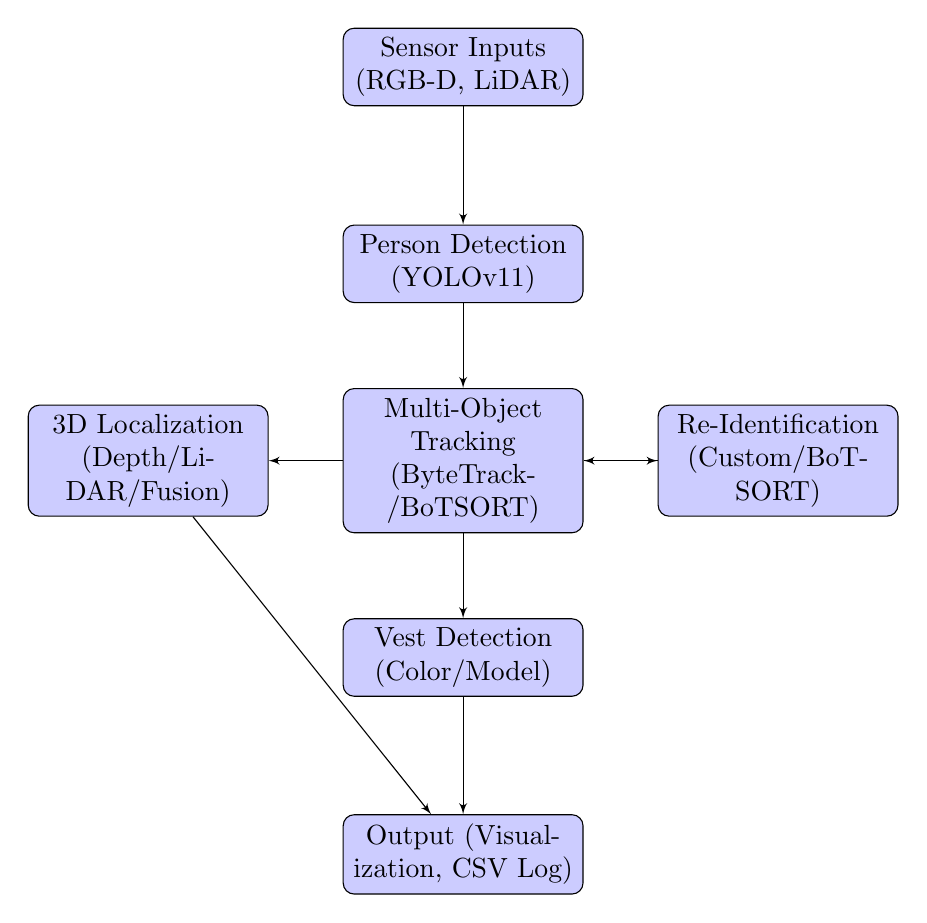
\begin{tikzpicture}[
        node distance=2.5cm,
        auto,
        block/.style={rectangle, draw, fill=blue!20, text width=8em, text centered, rounded corners, minimum height=.5em},
        line/.style={draw, -latex'}
    ]
        \node [block] (input) {Sensor Inputs (RGB-D, LiDAR)};
        \node [block, below of=input] (detection) {Person Detection (YOLOv11)};
        \node [block, below of=detection] (tracking) {Multi-Object Tracking (ByteTrack/BoTSORT)};
        \node [block, right of=tracking, node distance=4cm] (reid) {Re-Identification (Custom/BoTSORT)};
        \node [block, below of=tracking] (vest) {Vest Detection (Color/Model)};
        \node [block, left of=tracking, node distance=4cm] (localization) {3D Localization (Depth/LiDAR/Fusion)};
        \node [block, below of=vest] (output) {Output (Visualization, CSV Log)};

        \path [line] (input) -- (detection);
        \path [line] (detection) -- (tracking);
        \path [line] (tracking) -- (reid);
        \path [line] (reid) -- (tracking);
        \path [line] (tracking) -- (vest);
        \path [line] (tracking) -- (localization);
        \path [line] (vest) -- (output);
        \path [line] (localization) -- (output);
    \end{tikzpicture}
    \caption{System Architecture Diagram.}
    \label{fig:architecture}
\end{figure}

\section{System Design and Algorithms}
\subsection{Object Detection}
The choice of the nano version (`yolo11n.pt`) was driven by the need for high processing speed (FPS) to achieve real-time performance. While larger YOLO models offer higher accuracy, their computational cost is prohibitive for this application. YOLOv11n provides an excellent trade-off between speed and accuracy.\\

The `ultralytics` Python library is used to load the pre-trained model. In the main processing loop, the `model.track()` method is called on each frame. Detections are filtered to only include the "person" class (class ID 0) and are further filtered by a confidence threshold of 0.5 to discard low-certainty detections, thus reducing false positives.

\subsection{Multi-Object Tracking}
The system supports two different tracking algorithms, selectable via a command-line argument.
\subsubsection{ByteTrack}
A highly efficient tracker that challenges the common practice of discarding low-confidence detections. It retains all detection boxes and separates them into high- and low-confidence groups. It first matches high-confidence boxes to existing tracks. Then, it attempts to match the low-confidence boxes to unmatched tracks, effectively recovering objects during occlusion or motion blur. This makes it robust against missed detections without requiring complex appearance models.\\

On the advantages: high performance, computationally inexpensive, and effective at reducing missed tracks; as for disadvantages, it relies purely on motion prediction (Kalman filter) and bounding box overlap, so it can be prone to ID switches during long or complex occlusions where appearance is the only distinguishing factor.

\subsubsection{BoTSORT}
An enhanced version of the classic SORT (Simple Online and Realtime Tracking) algorithm. It integrates appearance information from a Re-ID model directly into its matching cascade, making it more robust than trackers that only use motion models.\\

On the advantages: higher tracking accuracy and fewer ID switches compared to ByteTrack, especially in crowded scenes or during prolonged occlusions; as for disadvantages, higher computational cost due to the need to compute appearance embeddings for matching.

\subsection{Advanced Person Re-Identification (Re-ID)}
Re-ID is crucial for maintaining consistent identities when a person is lost and later redetected.
\subsubsection{Custom Appearance Embedding with ResNet-18}
A custom Re-ID mechanism was implemented to provide robust tracking even when using a simple tracker like ByteTrack. ResNet-18, a deep convolutional neural network pre-trained on ImageNet, was chosen as the feature extractor. It is a well-established architecture that provides rich, discriminative features suitable for appearance matching, while being less computationally intensive than deeper networks like ResNet-50.\\

For each detected person, the cropped bounding box image is passed through the network to obtain a 512-dimensional feature vector (the "embedding"). When a track is lost, its last known embedding is stored. For newly detected tracks, their embeddings are compared against those of recently lost tracks using \textbf{cosine similarity}.\\

\begin{lstlisting}[caption={Core logic for generating appearance embeddings from `reid.py`.}, label={lst:reid}]
def get_appearance_embedding(person_image):
    # ... model initialization ...
    try:
        # Convert numpy image (from OpenCV) to PIL Image
        pil_image = Image.fromarray(cv2.cvtColor(person_image, cv2.COLOR_BGR2RGB))

        # Preprocess the image and add a batch dimension
        input_tensor = preprocess(pil_image)
        input_batch = input_tensor.unsqueeze(0).to(_device)

        # Get the feature embedding
        with torch.no_grad():
            embedding = _model(input_batch)

        # Flatten the embedding and convert to a numpy array
        return embedding.squeeze().cpu().numpy()
    except Exception as e:
        # ... error handling ...
        return None
\end{lstlisting}

The customization of threshold in Re-ID is a critical parameter for balancing the risk of incorrect merges versus missed re-identifications.

\subsection{3D Localization}
The system provides three methods for 3D localization, leveraging the available sensor data.

\subsubsection{RGB-D Camera Localization}
This method uses the pinhole camera model to deproject a 2D pixel coordinate into 3D space. The depth value $Z$ is read from the depth image at the center of the person's bounding box. The 3D coordinates $(X, Y, Z)$ in the camera frame are then calculated using the camera's intrinsic parameters (focal lengths $f_x, f_y$ and principal points $c_x, c_y$):
\begin{align*}
    X &= (u - c_x) \cdot Z / f_x \\
    Y &= (v - c_y) \cdot Z / f_y
\end{align*}

This method is computationally very fast and provides accurate depth information at close ranges (\textgreater 5 meters). However, its accuracy degrades significantly with distance, and it can fail on reflective or dark surfaces.\\

\begin{lstlisting}[caption={Deprojection logic from `localization.py`.}, label={lst:depth_loc}]
def get_3d_position(box, depth_image, K):
    # Get the center of the bounding box
    cx = int((box[0] + box[2]) / 2)
    cy = int((box[1] + box[3]) / 2)

    # Get depth value and convert to meters
    depth_in_mm = depth_image[cy, cx]
    if depth_in_mm == 0: return 0, 0, 0
    depth_in_m = depth_in_mm / 1000.0

    # Camera intrinsics
    fx, fy, px, py = K[0, 0], K[1, 1], K[0, 2], K[1, 2]

    # Deproject 2D point to 3D
    x_cam = (cx - px) * depth_in_m / fx
    y_cam = (cy - py) * depth_in_m / fy
    z_cam = depth_in_m

    return x_cam, y_cam, z_cam
\end{lstlisting}

\subsubsection{LiDAR Localization}
A more sophisticated and complex pipeline involving RANSAC for plane segmentation and DBSCAN for clustering. \\

The \textbf{RANSAC} (Random Sample Consensus) algorithm is used to robustly identify the dominant ground plane in the point cloud, which is then removed. This is critical for isolating points belonging to objects from the ground; then LiDAR points are transformed to the camera frame and projected onto the 2D image plane. Only points that fall within a person's 2D bounding box are retained, \textbf{DBSCAN} (Density-Based Spatial Clustering of Applications with Noise) is applied to these culled points; later, the median depth of the points in the largest cluster is used as the final depth estimate. The median is used instead of the mean to be robust against outliers.\\

This algorithm is effective because it can find non-linearly shaped clusters and is robust to noise. It groups the points that likely belong to the person. The largest cluster is selected as the most reliable representation of the person. This method is more accurate than the depth camera at longer ranges (\textgreater 5 meters) and is unaffected by lighting conditions. However, it is more computationally intensive, and the sparsity of LiDAR data can sometimes limit its precision.

\begin{lstlisting}[caption={Key steps in the LiDAR localization pipeline from lidar\_utils.py}, label={lst:lidar\_loc}]
def get_3d_position_from_lidar(box_2d, point_cloud, K, T_cam_lidar):
    # ... preprocessing ...
    # Remove ground plane to focus on objects above ground
    non_ground_cloud = remove_ground_plane(filtered_cloud)
    # ... transform points to camera frame ...
    # ... project 3D points to 2D and filter by bounding box ...
    
    # Advanced Depth Estimation using Clustering
    if points_in_box.shape[0] >= 3:
        clusters = cluster_points_in_box(points_in_box)
        if clusters:
            # Find the largest cluster (most reliable)
            largest_cluster_idx = max(clusters, key=len)
            cluster_points = points_in_box[largest_cluster_idx]
            # Use median depth of the largest cluster
            final_depth = np.median(cluster_points[:, 2])
    # ... fallback logic and final deprojection ...
    return x_cam, y_cam, z_cam
\end{lstlisting}

\subsubsection{Sensor Fusion}
The fusion strategy is a pragmatic approach that leverages the strengths of each sensor. It dynamically adjusts its trust in each sensor based on the measured distance, where their respective accuracies are known to be best.\\

\begin{lstlisting}[caption={Sensor fusion logic from \texttt{lidar\_utils.py}}, label={lst:fusion}]
def fuse_depth_and_lidar(...):
    depth_pos = get_3d_position(...)
    lidar_pos = get_3d_position_from_lidar(...)
    
    if (depth_pos != (0, 0, 0)) and (lidar_pos != (0, 0, 0)):
        depth_distance = depth_pos[2]
        # Weight based on distance
        if depth_distance < 5.0:  # < 5 meters, prefer depth
            weight_depth, weight_lidar = 0.7, 0.3
        else:  # >= 5 meters, prefer LiDAR
            weight_depth, weight_lidar = 0.3, 0.7
            
        fused_x = weight_depth * depth_pos[0] + weight_lidar * lidar_pos[0]
        # ... same for y and z ...
        return fused_x, fused_y, fused_z
    
    # Fallback to individual sensors
    elif depth_pos != (0, 0, 0): return depth_pos
    elif lidar_pos != (0, 0, 0): return lidar_pos
    else: return 0, 0, 0
\end{lstlisting}

The system calculates the 3D position from both the depth camera and LiDAR. If both are successful, it computes a weighted average. For distances less than 5 meters, the weights are 70\% for the depth camera and 30\% for LiDAR. For distances of 5 meters or more, the weights are inverted. The system also includes a crucial fallback mechanism: if one sensor fails, it uses the result from the other, ensuring maximum availability.

\subsection{Safety Vest Detection}
Two distinct methods are provided for vest detection.

\subsubsection{Color-Based Detection}
It first undergoes enhancement to normalize for lighting variations using \textbf{adaptive gamma correction} and \textbf{CLAHE} (Contrast Limited Adaptive Histogram Equalization). The enhanced image is then converted to the HSV color space, which is more robust to lighting changes than RGB. A binary mask is created for a predefined range of yellow hues. Morphological operations (erosion and dilation) are applied to remove noise from this mask. A vest is detected if the percentage of yellow pixels exceeds the defined threshold. This approach is extremely fast and simple to implement; however, it is highly sensitive to ambient lighting and can be easily confused by other yellow objects.\\

\begin{lstlisting}[caption={Image enhancement pipeline from `vision.py`.}, label={lst:color_vest}]
def detect_yellow_vest(person_image, threshold=5.0):
    # Extract upper body region
    upper_half = extract_upper_body_roi(person_image)
    # Apply gamma correction
    upper_half = adaptive_gamma_correction(upper_half)
    # Enhance with CLAHE
    upper_half = enhance_yellow_with_clahe(upper_half)

    # HSV validation
    mask_hsv, yellow_percentage_hsv = validate_hsv_color(upper_half)
    
    yellow_percentage = yellow_percentage_hsv * 100
    return yellow_percentage > threshold, mask_hsv, yellow_percentage_hsv
\end{lstlisting}

\subsubsection{Model-Based Detection}
MobileNetV2 was chosen for its efficiency, making it suitable for real-time classification without a significant performance penalty. It provides a much more robust solution than color thresholding by learning features associated with the shape and context of a vest, not just its color. The detection module loads a MobileNetV2 model where the final classification layer has been replaced with one that outputs two classes (vest, no-vest). The cropped person image is resized to 224x224 and normalized before being fed to the model for prediction. This approach increases accuracy and robustness to lighting conditions. Its main drawbacks are the need for a pre-trained model and its higher computational cost compared to the color-based method. \\

\begin{lstlisting}[caption={Prediction function from `vest\_classifier.py`.}, label={lst:model_vest}]
def predict(self, person_image):
    # Convert BGR image to RGB
    rgb_image = cv2.cvtColor(person_image, cv2.COLOR_BGR2RGB)

    # Apply transformations and add a batch dimension
    input_tensor = self.transform(rgb_image).unsqueeze(0).to(self.device)

    with torch.no_grad():
        output = self.model(input_tensor)
        # Apply softmax to get probabilities
        probabilities = torch.nn.functional.softmax(output, dim=1)
        confidence, predicted_class = torch.max(probabilities, 1)

    is_vest = predicted_class.item() == 1
    return is_vest, confidence.item()
\end{lstlisting}

\section{Testing Environment}
A \href{https://github.com/Gioyik/xtrack_sensys_2025/blob/main/TESTING_PLAN.md}{testing plan} has been laid out inside the repository source code. The following hardware has been put to the test.

\subsection{Hardware Configurations}

\begin{table}[h!]
\centering
\resizebox{\textwidth}{!}{%
\begin{tabular}{|l|l|l|l|}
\hline
\textbf{System} & \textbf{CPU} & \textbf{RAM} & \textbf{GPU} \\
\hline
System 1 (Gaming Laptop) & Intel i7-10750H @ 2.60GHz (6C/12T) & 15.8 GB & NVIDIA GTX 1650 Ti (4GB) + Intel UHD \\
\hline
System 2 (Ultrabook) & Intel i7-1355U @ 1.70GHz (10C/12T) & 16.0 GB (15.7 GB usable) & Intel Iris Xe Graphics \\
\hline
System 3 (Apple M1 MacBook) & Apple M1 (8 cores) & 8 GB unified & Apple M1 (8 GPU cores) \\
\hline
System 4 (Apple M2 Pro MacBook) & Apple M2 Pro (10 cores: 6P+4E) & 16 GB unified & Apple M2 Pro (16 GPU cores) \\
\hline
\end{tabular}%
}
\caption{Hardware configurations tested for benchmarking.}
\end{table}

\section{Results and Evaluation}
\subsection{Localization Method Performance}
Apple M2 Pro achieves the highest performance: \textbf{66.40 FPS} with fusion (24\% faster than M1). Apple Silicon systems dramatically outperform Intel systems (6x+ faster), and localization works properly only on System 1, System 3, and System 4.

\subsection{Tracker Algorithm Comparison}
ByteTrack demonstrates superior performance across all hardware platforms with better track continuity and computational efficiency. The M2 Pro shows the highest absolute performance with ByteTrack achieving 65.93 FPS, a 23\% improvement over M1 and 6.6x improvement over the best Intel system.

\subsection{Vest Detection Methods}
\textbf{Color-based vs Model-based Detection:}
\begin{itemize}
    \item Color-based: 32.9\% detection rate, faster processing
    \item Model-based: 100\% detection rate, 56ms additional processing time
\end{itemize}

Model-based detection achieves perfect detection but adds significant computational overhead (68.69ms vs 3.35ms for vest processing).

\subsection{Frame Skipping Optimization}
Apple Silicon systems maintain excellent performance with minimal benefit from frame skipping. The M2 Pro shows interesting vest detection improvements with moderate skipping (1--2 frames), but excessive skipping (4+ frames) degrades tracking quality even on high-performance hardware.

\subsection{Vest Detection Threshold Analysis}
Lower thresholds increase detection sensitivity but can severely impact performance on some hardware configurations.

\begin{itemize}
    \item 3\% threshold: 2.92 FPS (System 1), 39.7\% detection rate
    \item 5\% threshold: 12.35 FPS (System 1), 32.9\% detection rate
    \item 8\% threshold: 11.51 FPS (System 1), 25.0\% detection rate
    \item 12\% threshold: 11.53 FPS (System 1), 13.0\% detection rate
\end{itemize}

\subsection{Peak Performance Achievement}
The Apple M2 Pro system establishes new performance benchmarks:

\begin{itemize}
    \item M2 Pro System: 66.40 FPS (Sensor Fusion)
        \item M2 Pro achieves \textbf{6.7x faster} processing than the best Intel system
        \item M2 Pro is \textbf{24\% faster} than M1 on identical workloads
    \item M1 System: 53.43 FPS (Depth Camera)
    \item Intel Gaming: 9.88 FPS baseline
    \item Intel Ultrabook: 8.53 FPS baseline
\end{itemize}

\appendix
\section{Links}

The source code and supplementary materials for this work are available at the following repository:

\begin{itemize}
    \item Project Repository: \href{https://github.com/Gioyik/xtrack_sensys_2025}{https://github.com/Gioyik/xtrack_sensys_2025}
    \item Video Presentation: \href{https://tubcloud.tu-berlin.de/s/oc8aTzg3sCLFqn2}{tubCloud}
\end{itemize}

\end{document}
